% questions.tex —— 1977 年·山西卷 · 题目内容片段（无答案）
% 由 tools/generate_projects.py 依来源总账自 1977/1977_数学真题_山西_试题.md 生成，勿手改（改源 MD 后重跑）


\gkpart{数学试题解}

\begin{gktip}
\textbf{来源说明}：本题面依据固定源 PDF《山西1977年高考数学试题解》第 1—4 页逐题转录；固定源是题面与解答连续出现的扫描材料（书籍页码 36—39），不是无答案试卷。正式题为第 1—8 题，末尾“参考题”两题不计入题量。原卷题号体例混用：第 1 题印作“1、”，第 2—8 题印作“二、”至“八、”，本卷统一重排为阿拉伯数字；原卷第 2 题三个小题印作“1．”“2．”“3．”，按本库规范重排为（1）（2）（3）。原卷函数记号 Lg、Ln、Log、Sin、Cos 在数学式中按原样保留（数学式中排作反斜杠 operatorname 形式），tg 同理。
\end{gktip}

\par\medskip

\begin{question}
\gkti{1}\textbf{（20 分）} 化简下列各题：

（1） $\dfrac{1}{\sqrt2+1}-\dfrac{1}{\sqrt2-1}$；

（2） $\dfrac{(a^2-b^2)^3}{a^3+b^3}\div\dfrac{(b+a)^2}{a^2-ab+b^2}\times\dfrac{1}{(b-a)^3}$；

（3） $\dfrac{2\operatorname{Lg}6-\operatorname{Lg}3}{1+\frac12\operatorname{Lg}0.36+\frac13\operatorname{Lg}8}$；

（4） $\dfrac{x^4+x^2+1}{x^3-1}+\dfrac{x(x-2)-2(x-2)}{x^2-3x+2}$.

\end{question}
\begin{question}
\gkti{2}\textbf{（20 分）} 作下列各题：

\begin{gktip}
\textbf{题号说明}：原卷本题三个小题印作“1．”“2．”“3．”，本卷按小问格式重排为（1）（2）（3），未增删题干。
\end{gktip}

（1） 当 $a\text{、}b\text{、}c>0$ 时，求证：$\operatorname{Log}_a b\cdot\operatorname{Log}_b c\cdot\operatorname{Log}_c a=1$。

\begin{gktip}
\textbf{源注}：原卷第二、三个因子的真数 $c\text{、}a$ 排印为上标位置（形似 $\operatorname{Log}_b^c$、$\operatorname{Log}_c^a$）；按源解答的换底公式 $\operatorname{Log}_a b=\dfrac{\operatorname{Lg}b}{\operatorname{Lg}a}$ 确认其为真数，本卷按真数转录。
\end{gktip}

（2） 已知 $y=\operatorname{Lg}\dfrac{1}{1-\sqrt{1-x}}$，求定义域。

（3） 汽车往返甲乙两地之间，上行速度为 30 公里/小时，下行速度为 60 公里/小时。求往返平均速度。

\Needspace{0.4\textheight}
\end{question}
\begin{question}
\gkti{3}\textbf{（10 分）} 试证梯形的中位线平行于两底，且等于两底和的一半。

已知：如图，梯形 $ABCD$，$AD\parallel BC$，$M\text{、}N$ 分别为 $AB\text{、}DC$ 之中点。

求证：

（1） $MN\parallel AD$，$MN\parallel BC$；

（2） $MN=\dfrac12(AD+BC)$。

\begin{gktip}
原源 PDF 第 2 页附有梯形与中位线 $M\text{、}N$ 及辅助线 $DM$ 延长线示意图；LaTeX 版按源图重绘。
\end{gktip}
\nopagebreak[4]
\begin{center}% 1977 年山西卷第三题：梯形 ABCD（A 左上、D 右上、B 左下、C 右下，上底 AD 短、下底 BC 长），
% M、N 分别为腰 AB、DC 中点，MN 为中位线（实线）；辅助线：DM 延长交 CB 的延长线于 E（虚线 D-M-E），
% E—B 沿底边延长线（虚线）（按源卷第 2 页布局）
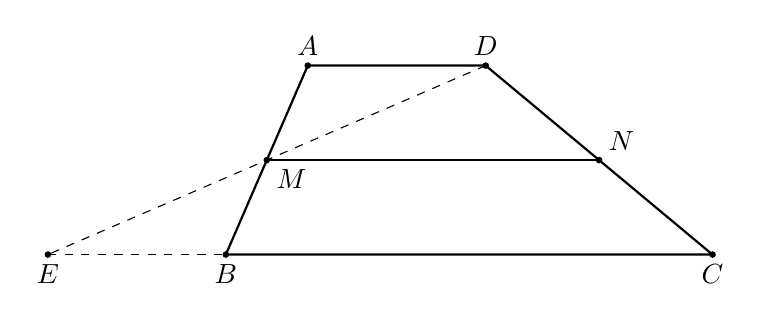
\begin{tikzpicture}[scale=1.0]
  \coordinate (A) at (0,2.4);
  \coordinate (D) at (2.26,2.4);
  \coordinate (B) at (-1.04,0);
  \coordinate (C) at (5.14,0);
  \coordinate (M) at (-0.52,1.2);
  \coordinate (N) at (3.7,1.2);
  \coordinate (E) at (-3.3,0);
  \draw[thick] (A)--(B)--(C)--(D)--cycle;
  \draw[thick] (M)--(N);
  \draw[dashed] (D)--(M)--(E);
  \draw[dashed] (E)--(B);
  \fill (A) circle (1.2pt) node[above] {$A$};
  \fill (D) circle (1.2pt) node[above] {$D$};
  \fill (B) circle (1.2pt) node[below] {$B$};
  \fill (C) circle (1.2pt) node[below] {$C$};
  \fill (M) circle (1.2pt) node[below right] {$M$};
  \fill (N) circle (1.2pt) node[above right] {$N$};
  \fill (E) circle (1.2pt) node[below] {$E$};
\end{tikzpicture}
\end{center}
\nopagebreak[4]
\end{question}
\begin{question}
\gkti{4}\textbf{（10 分）} 有一块形状为直角三角形的白铁皮，其一直角边和斜边分别为 6 dm 和 10 dm。若从这块白铁皮剪一块最大圆材料，求这圆材料的面积有多大？（$\pi$ 取 3.14）

\end{question}
\begin{question}
\gkti{5}\textbf{（10 分）} 证明恒等式：

\nopagebreak[4]
\[
\frac{1+\operatorname{Sin}(180^\circ-\alpha)-\operatorname{Cos}(180^\circ+\alpha)+\operatorname{Sin}2\alpha}
{1-\operatorname{Sin}(180^\circ+\alpha)+\operatorname{Cos}(\alpha-360^\circ)}
=\operatorname{Sin}\alpha+\operatorname{Cos}\alpha.
\]

\end{question}
\begin{question}
\gkti{6}$\triangle ABC$ 的三个内角是 $\alpha\text{、}\beta\text{、}\gamma$，而 $\operatorname{tg}\alpha\text{、}\operatorname{tg}\beta$ 是方程 $x^2-5x+6=0$ 的两个根。求 $\gamma$。

\end{question}
\begin{question}
\gkti{7}\textbf{（8 分）} 抛物线的顶点在原点，对称轴为 $y$ 轴，过点 $(1,-1)$，求抛物线方程，焦点坐标，准线方程，开口方向。

\Needspace{0.4\textheight}
\end{question}
\begin{question}
\gkti{8}\textbf{（12 分）} 当 $k$ 取何值时，直线 $kx-y-3=0$ 与圆 $2x^2+2y^2-9=0$ 相切，并求出切点坐标。

\begin{gktip}
\textbf{参考题}
\end{gktip}

\textbf{参考题 1．} 已知 $f(x)=x\operatorname{Ln}(2-x)+\sqrt{1+3x^2}$，求 $f'(1)$。

\textbf{参考题 2．} 一水库的水闸为一等腰梯形，上底为 8 米，下底为 4 米，高为 10 米。求当水面与上底相齐时水闸所受的压力。（已知水的比重为 1 吨重/立方米）

\begin{gktip}
原源 PDF 第 4 页附有水闸（倒梯形）与水深 $x$ 处面积元示意图；LaTeX 版按源图重绘。
\end{gktip}
\nopagebreak[4]
\begin{center}% 1977 年山西卷参考题 2：水库水闸（等腰梯形，上底 8 米、下底 4 米、高 10 米），
% 水面与上底相齐（顶部水平线为水面线）；水深 x 米处取水平面积元（阴影条，高 dx），
% 左侧标 x 米（水面到面积元的深度）、右侧标总高 10 米、底部标下底 4 米（按源卷第 4 页布局）
\begin{tikzpicture}[scale=0.86,>=stealth]
  % 水闸（倒梯形：上底宽、下底窄）
  \coordinate (TL) at (0,3);
  \coordinate (TR) at (5,3);
  \coordinate (BL) at (1,0);
  \coordinate (BR) at (4,0);
  \draw[thick] (TL)--(BL)--(BR)--(TR)--cycle;
  % 水面线（与上底相齐，两端延伸）
  \draw[thick] (-0.5,3)--(5.7,3);
  % 深度 x 处的水平面积元（阴影条，高 dx）
  \draw (0.72,2.15) rectangle (4.28,2.35);
  \foreach \x in {0.85,1.15,...,4.05}{
    \draw (\x,2.15)--(\x+0.2,2.35);
  }
  \node[right] at (4.55,2.25) {$dx$};
  % 左侧：x 米（水面到面积元）
  \draw[<->] (-0.25,3)--(-0.25,2.15);
  \node[left,rotate=90,anchor=center] at (-0.42,2.6) {$x\,\text{米}$};
  % 右侧：总高 10 米
  \draw[<->] (5.45,3)--(5.45,0);
  \node[right,rotate=90,anchor=center] at (5.62,1.5) {$10\,\text{米}$};
  % 底部：下底 4 米
  \draw[<->] (1,-0.4)--(4,-0.4);
  \node[below] at (2.5,-0.45) {$4\,\text{米}$};
  % 顶部：上底 8 米
  \draw (0,3.12)--(0,3.3);
  \draw (5,3.12)--(5,3.3);
  \draw[<->] (0,3.25)--(5,3.25);
  \node[above] at (2.5,3.28) {$8\,\text{米}$};
\end{tikzpicture}
\end{center}
\nopagebreak[4]

\end{question}